\chapter{Experimentos e Resultados}
\label{cap:texto}

Neste capítulo, detalharemos a configuração dos testes realizados e apresentaremos os resultados obtidos. No que concerne ao ambiente de simulação, empregamos a Engine V-Rep ~\cite{Rohmer2013} com o motor físico Bullets v2.8. Para a emissão de comandos ao simulador, tais como o início e a interrupção da simulação, utilizamos a biblioteca Python do V-Rep, que implementa a comunicação com o simulador baseada em Sockets. Adicionalmente, para a obtenção do estado (posição, orientação, IMU, etc.) e o fornecimento de comandos ao robô, recorremos ao Robot Operating System (ROS), que estabelece um canal de comunicação assíncrona fundamentado em tópicos (arquitetura publishers/subscribers). A título de ilustração desta comunicação, citamos o tópico dos ângulos dos atuadores, onde os valores são gerados e publicados pelo controlador, sendo subsequentemente consumidos pelo script em Lua no simulador para aplicação no robô.

\section{Simulações}

Nas simulações do controlador, utilizou-se um intervalo de tempo ($dt$) de 50 ms, o padrão do V-Rep, proporcionando um framerate suficiente para execução dos comandos. Uma das vantagens do controlador proposto é a capacidade de calibrar os parâmetros das equações que definem a cinemática do robô. Para tal, as variáveis foram divididas em dois grupos: o primeiro, apresentado na Tabela~\ref{tab:grupo1}, contém variáveis de ajuste mínimo ou nulo durante a calibração, e o segundo, na Tabela~\ref{tab:grupo2}, inclui variáveis ajustáveis para otimizar o desempenho cinemático do robô, conforme os critérios de avaliação.

\begin{table}[H]
\centering
\caption{Valores do grupo de variáveis 1.}
\label{tab:grupo1}
\begin{tabular}{lc}
\hline
Parâmetro & Valor \\
\hline
$\sigma_{tanh}$ & 5 \\
$\sigma_{sino}$ & 0.5 \\
$K_p$ & 0.3 \\
$h_{hip}$ & 17 \\
\hline
\end{tabular}
\end{table}

\begin{table}[H]
\centering
\caption{Valores do grupo de variáveis 2.}
\label{tab:grupo2}
\begin{tabular}{lc}
\hline
Parâmetro & Valor \\
\hline
$T_{passo}$ & 0.35 \\
$l_{hip}$ & 3 \\
$u_{foot}$ & 2.5 \\
$d_{feet}$ & 1.2 \\
$\theta_{Maxyall}$ & 15 \\
\hline
\end{tabular}
\end{table}

As métricas utilizadas para avaliar o controlador são dadas a seguir:

\begin{itemize}
    \item \textbf{Duração}: Tempo de duração em segundos do episódio até o bípede cair ou chegar ao objetivo.
    \item \textbf{Média da variação da orientação do torso em Roll e Pitch (IMU)}: Esta métrica nos dá a informação do quanto a orientação o torso variou (em graus) em relação aos eixos X e Y. Consideramos o cenário ótimo quando não há nenhuma variação, ou seja, a média será 0. Vale destacar que essa variação é absoluta, por exemplo, caso a leitura de orientação do torso seja -5 iremos computar uma variação de 5 graus, ignorando o sentido da rotação.
    \item \textbf{Desvio padrão da variação angular do torso}: Essa medida nos permite definir um intervalo de confiança para a média da variação da orientação descrita acima.
    \item \textbf{Distância}: Distância percorrida em metros pelo bípede durante o episódio (também mostraremos essa distância ao longo do tempo).
\end{itemize}

Os parâmetros do Grupo 1 foram ajustados conforme os objetivos descritos na metodologia, enquanto os parâmetros do Grupo 2, listados na Tabela~\ref{tab:grupo2}, foram determinados através da calibração do robô. Inicialmente, todos os parâmetros do Grupo 2 foram definidos como zero e o controlador de alto nível foi configurado para o estado "Caminhando". Com essa configuração inicial, podemos começar o processo de calibração:

\begin{enumerate}
    \item Primeiro precisamos definir $T_{passo}$, o tempo de um passo e portanto metade do ciclo de caminhada. Vale destacar que teremos que encontrar os valores apropriados para cada um dos demais parâmetros cada vez que $T_{passo}$ for alterado. Inicialmente foi realizada a calibração com o valor 1, reduzindo até 0.35. Pelo padrão observado durante a calibração, quanto menor for este valor menos precisaremos deslocar lateralmente o torso (ou posição do CoM), contando que haverá maiores quantidades de momento aplicados ao corpo, ou considerando um determinado estado onde o ZMP não está sobre a SC, o tombamento acontecerá de forma gradual dando tempo do próximo passo ser iniciado e possivelmente corrigir as perturbações.
    
    \item Agora iremos ajustar o $l_{hip}$ (deslocamento lateral do quadril) e $u_{foot}$ (altura máxima do pé de balanço), primeiro ajustamos o $l_{hip}$ aumentando gradualmente o seu valor até que o bípede comece a produzir um tombamento lateral, isso se dá pelo fato do ZMP estar extrapolando a SC e portanto representa o valor máximo que esse parâmetro pode ter, depois iremos reduzir um pouco até que o bípede não apresente mais tombamento lateral, por fim iremos aumentar gradualmente $u_{foot}$ até que esteja visível que o pé de balanço está perdendo contato com o chão. Com isso definimos os parâmetros necessários para o robô marchar.
    
    \item Por último iremos definir $d_{feet}$ (distância do passo) e $\theta_{Maxyall}$ (rotação máxima em Yall durante o passo), similar aos demais parâmetros os valores foram obtidos aumentando gradualmente até que o bípede apresente perturbações e reduzindo até que a marcha esteja estável. Vale destacar que quanto maiores estes valores, mais rapidamente o bípede irá se deslocar ou rotacionar.
\end{enumerate}

Após a calibração da marcha, foram executadas 40 simulações onde o ponto objetivo foi posicionado a 1 metro à esquerda do robô, sendo esta uma distância de um pouco mais de 3 vezes a sua altura. Com isso, definimos a tarefa de rotacionar 90 graus na direção do alvo e caminhar uma distância suficiente para gerar desvios de trajetória.

% {{PLACE_HOLDER_FIGURA_5}}
% Figura 5
\begin{figure}[H]
  \centering
  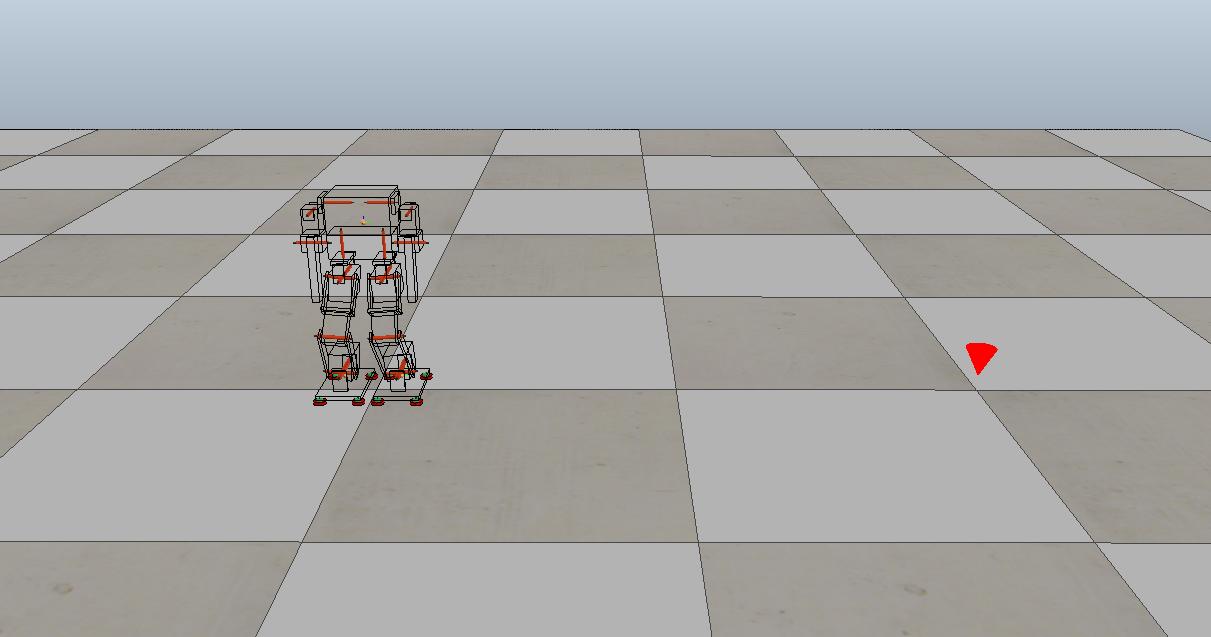
\includegraphics[width=0.7\textwidth]{./fig/fig5}
  \caption{Imagem da configuração inicial da simulação.}
  \label{fig:sim_config}
\end{figure}

Para ilustrar os resultados das simulações iremos utilizar gráficos de frequência (histograma) e variação ao longo do tempo. Em nenhuma das simulações o robô apresentou queda, fazendo com que em todas as vezes o objetivo fosse alcançado, como mostra a Figura~\ref{fig:distancias}. Além disso, as simulações apresentaram baixas variações na orientação, aproximadamente entre 1 e 1.5 em roll, e 0 e 1.1 em pitch, como mostra a Figura~\ref{fig:variacao} e Figura~\ref{fig:desvio}.

% {{PLACE_HOLDER_FIGURA_6}}
% Figura 6 (subfiguras)
\begin{figure}[H]
  \centering
  \subfigure[][Frequência das distâncias finais.]{
    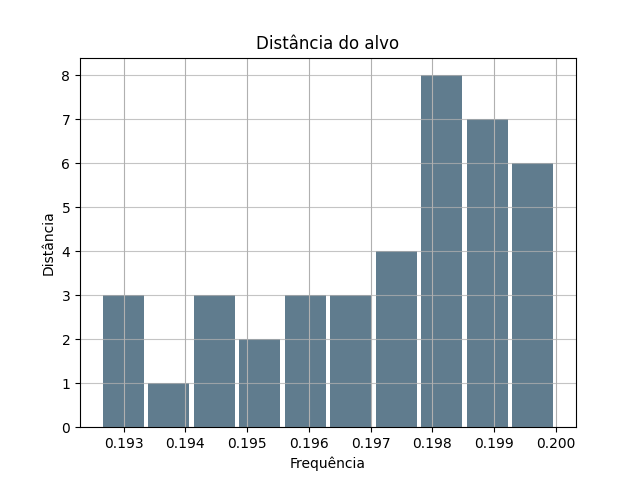
\includegraphics[width=0.45\textwidth]{./fig/fig6a}
    \label{fig:dist_freq}
  }
  \hspace{0.05\textwidth}
  \subfigure[][Variação dessas distâncias ao longo do tempo.]{
    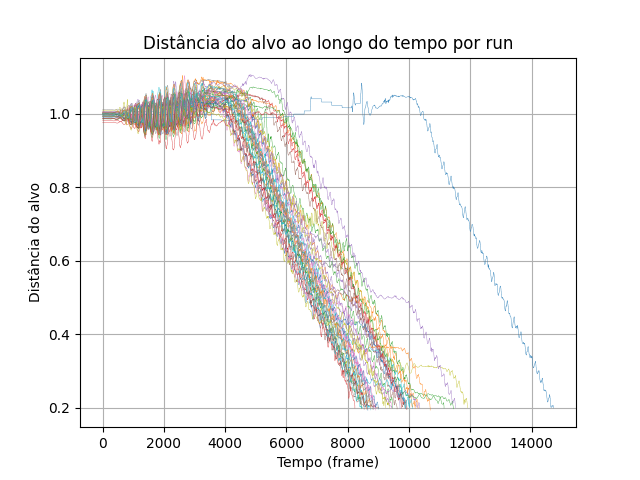
\includegraphics[width=0.45\textwidth]{./fig/fig6b}
    \label{fig:dist_tempo}
  }
  \caption{(a) indica a frequência das distâncias (em metros) do ponto objetivo no final da simulação, e (b) a variação dessas distâncias ao longo do tempo para cada simulação.}
  \label{fig:distancias}
\end{figure}

% {{PLACE_HOLDER_FIGURA_7}}
% Figura 7 (subfiguras)
\begin{figure}[H]
  \centering
  \subfigure[][Variação angular média em X (roll).]{
    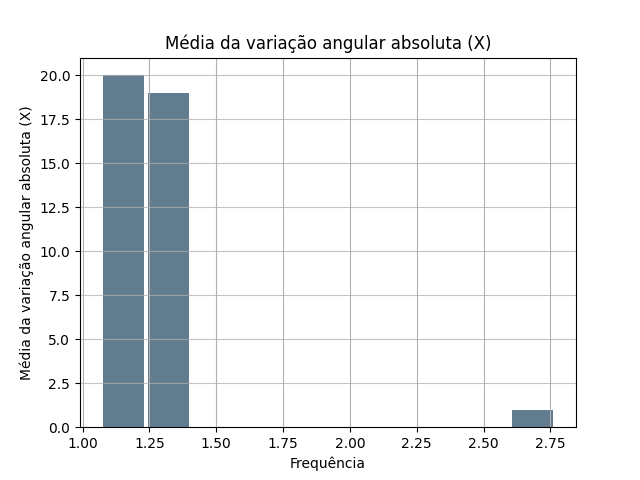
\includegraphics[width=0.45\textwidth]{./fig/fig7a}
    \label{fig:var_x}
  }
  \hspace{0.05\textwidth}
  \subfigure[][Variação em Y (pitch).]{
    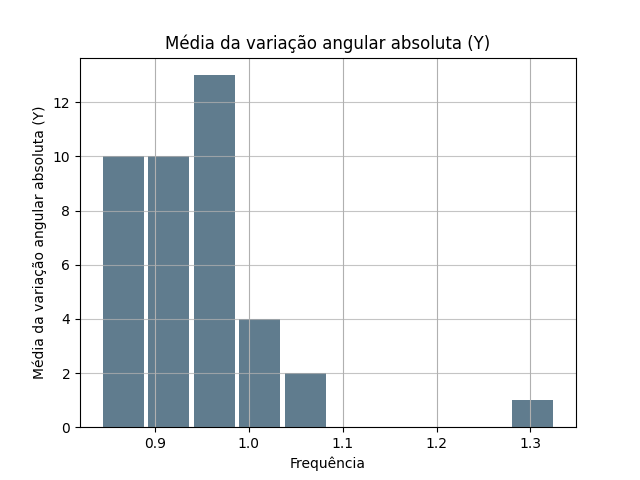
\includegraphics[width=0.45\textwidth]{./fig/fig7b}
    \label{fig:var_y}
  }
  \caption{Frequência dos intervalos definidos sobre os valores de variação angular média de cada simulação, medido em graus. (a) mostra a variação em X (roll) e (b) a variação em Y (pitch).}
  \label{fig:variacao}
\end{figure}

% {{PLACE_HOLDER_FIGURA_8}}
% Figura 8 (subfiguras)
\begin{figure}[H]
  \centering
  \subfigure[][Desvio padrão da variação em X (roll).]{
    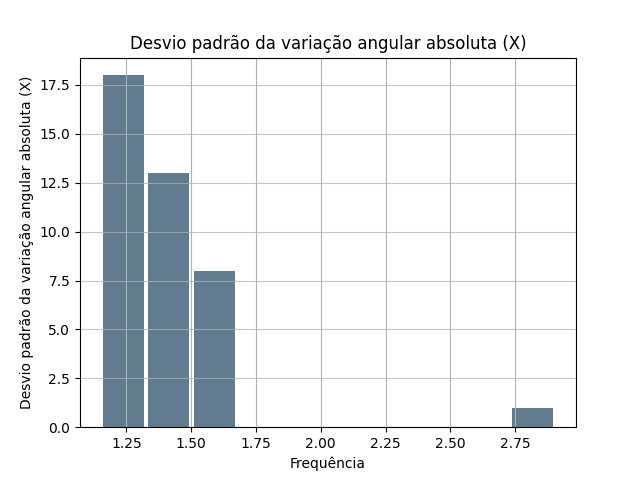
\includegraphics[width=0.45\textwidth]{./fig/fig8a}
    \label{fig:desvio_x}
  }
  \hspace{0.05\textwidth}
  \subfigure[][Desvio padrão em Y (pitch).]{
    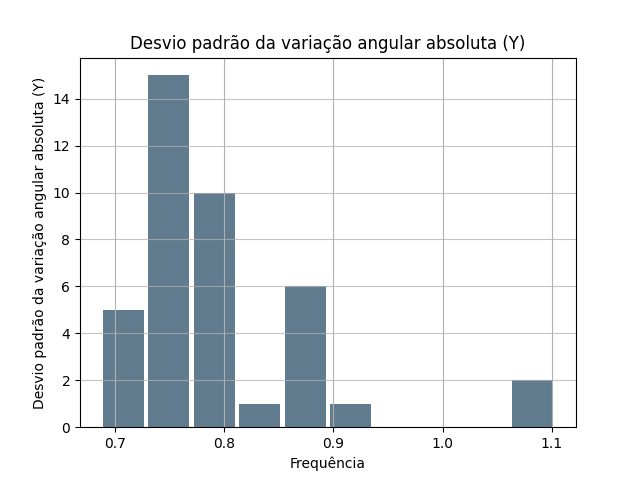
\includegraphics[width=0.45\textwidth]{./fig/fig8b}
    \label{fig:desvio_y}
  }
  \caption{Frequência dos intervalos definidos sobre os valores de desvio padrão da variação angular de cada simulação, medido em graus. (a) mostra o desvio da variação em X (roll) e (b) o desvio da variação em Y (pitch).}
  \label{fig:desvio}
\end{figure}

% {{PLACE_HOLDER_FIGURA_9}}
% Figura 9
\begin{figure}[H]
  \centering
  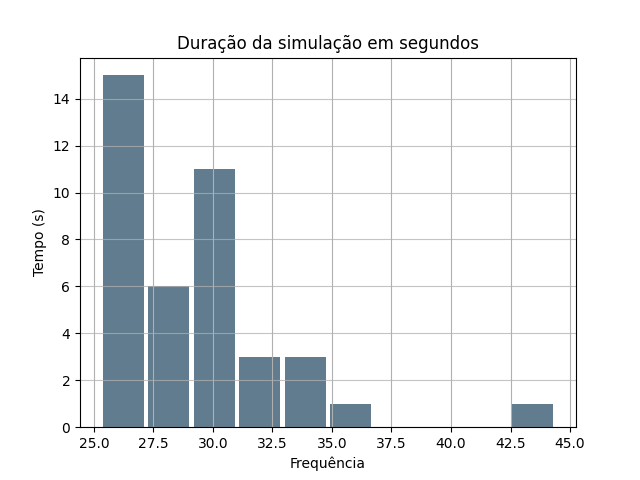
\includegraphics[width=0.7\textwidth]{./fig/fig9}
  \caption{Frequência da duração dos episódios em segundos.}
  \label{fig:duracao}
\end{figure}

\section{Discussões e Conclusão}
Com base nos experimentos realizados, os resultados obtidos demonstram que o controlador heurístico proposto é capaz de gerar padrões de caminhada estáveis e eficientes para o robô bípede simulado. Em todas as simulações realizadas, o robô foi capaz de atingir o objetivo sem apresentar quedas, evidenciando a robustez do método frente às condições testadas. As métricas de avaliação, como a baixa variação angular do torso e o desvio padrão reduzido dessas variações, indicam que o controlador proporciona uma marcha próxima ao comportamento esperado, com boa estabilidade e controle postural. Além disso, a abordagem baseada em funções heurísticas e parâmetros ajustáveis mostrou-se eficaz para a calibração do movimento, permitindo adaptações rápidas conforme as necessidades do experimento. Apesar dos bons resultados em ambiente simulado, ressalta-se que a sensibilidade a perturbações externas ainda é um desafio, sugerindo que futuras melhorias podem ser alcançadas com a incorporação de informações sensoriais em tempo real e estratégias de controle adaptativo. De modo geral, o controlador desenvolvido cumpre satisfatoriamente os objetivos propostos, servindo como uma base sólida para avanços futuros em controle de locomoção de robôs humanoides.



